\XtoCBlock{Biquad}
\label{block:Biquad}
\begin{figure}[H]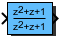
\includegraphics{Biquad}\end{figure} 

\begin{XtoCtabular}{Inports}
In & Input In(k)\tabularnewline
\hline
\end{XtoCtabular}


\begin{XtoCtabular}{Outports}
Out & Output Out(k)\tabularnewline
\hline
\end{XtoCtabular}

\begin{XtoCMaskParamTabular}{Mask Parameters}
\rowcolor[gray]{0.8}\textbf{Name} & \textbf{ID} & \textbf{Description}\tabularnewline\hline
b0 & 1 & Filter coefficient b0\tabularnewline
\hline
b1 & 2 & Filter coefficient b1\tabularnewline
\hline
b2 & 3 & Filter coefficient b2\tabularnewline
\hline
a0 & 4 & Filter coefficient a0\tabularnewline
\hline
a1 & 5 & Filter coefficient a1\tabularnewline
\hline
a2 & 6 & Filter coefficient a2\tabularnewline
\hline
ts\_fact & 7 & Multiplication factor of base sampling time (in integer format)\tabularnewline
\hline
\end{XtoCMaskParamTabular}

\subsubsection*{Description:}
Second order transfer function:

    H(z) = (b0.z\textsuperscript{2} + b1.z + b2) / (a0.z\textsuperscript{2} + a1.z + a2)

% include optional documentation file
\InputIfFileExists{\XcHomePath/Library/Filter/Doc/Biquad_Info.tex}{\vspace{1ex}}{}

\subsubsection*{Implementations:}
\begin{tabular}{l l}
\textbf{FiP16} & 16 Bit Fixed Point Implementation\tabularnewline
\textbf{FiP32} & 32 Bit Fixed Point Implementation\tabularnewline
\textbf{Float32} & 32 Bit Floating Point Implementation\tabularnewline
\textbf{Float64} & 64 Bit Floating Point Implementation\tabularnewline
\end{tabular}

\XtoCImplementation{FiP16}
\nopagebreak[0]

16 Bit Fixed Point Implementation

\begin{XtoCtabular}{Inports Data Type}
In & int16\tabularnewline
\hline
\end{XtoCtabular}

\begin{XtoCtabular}{Outports Data Type}
Out & int16\tabularnewline
\hline
\end{XtoCtabular}

\ifdefined \AddTestReports
\InputIfFileExists{\XcHomePath/Library/Filter/Doc/Test-Results/Test_Biquad_FiP16.tex}{}{}
\fi
\XtoCImplementation{FiP32}
\nopagebreak[0]

32 Bit Fixed Point Implementation

\begin{XtoCtabular}{Inports Data Type}
In & int32\tabularnewline
\hline
\end{XtoCtabular}

\begin{XtoCtabular}{Outports Data Type}
Out & int32\tabularnewline
\hline
\end{XtoCtabular}

\ifdefined \AddTestReports
\InputIfFileExists{\XcHomePath/Library/Filter/Doc/Test-Results/Test_Biquad_FiP32.tex}{}{}
\fi
\XtoCImplementation{Float32}
\nopagebreak[0]

32 Bit Floating Point Implementation

\begin{XtoCtabular}{Inports Data Type}
In & float32\tabularnewline
\hline
\end{XtoCtabular}

\begin{XtoCtabular}{Outports Data Type}
Out & float32\tabularnewline
\hline
\end{XtoCtabular}

\ifdefined \AddTestReports
\InputIfFileExists{\XcHomePath/Library/Filter/Doc/Test-Results/Test_Biquad_Float32.tex}{}{}
\fi
\XtoCImplementation{Float64}
\nopagebreak[0]

64 Bit Floating Point Implementation

\begin{XtoCtabular}{Inports Data Type}
In & float64\tabularnewline
\hline
\end{XtoCtabular}

\begin{XtoCtabular}{Outports Data Type}
Out & float64\tabularnewline
\hline
\end{XtoCtabular}

\ifdefined \AddTestReports
\InputIfFileExists{\XcHomePath/Library/Filter/Doc/Test-Results/Test_Biquad_Float64.tex}{}{}
\fi
